\documentclass[14pt]{extarticle}
\usepackage{fontspec}
\usepackage{polyglossia}
\usepackage{amsmath}
\usepackage{amssymb}
\usepackage{xcolor}
\usepackage{fancyhdr}
\usepackage{graphicx}
\usepackage{listings}
\usepackage[most]{tcolorbox}
% \usepackage{setspace}
\usepackage{pifont}
\usepackage{enumitem}
\usepackage{titlesec}
\usepackage[bottom]{footmisc}
\usepackage{titling}
\usepackage{minted}
\usepackage{etoolbox}
\usepackage{array}
\usepackage{extsizes}
\usepackage{float}
\usepackage{booktabs}
\usepackage{hyperref}
\usepackage[onehalfspacing]{setspace}
\usepackage[a4paper, top=2.7cm, bottom=2.7cm, left=2.5cm, right=2.5cm, headheight=1.5cm, headsep=0.5cm]{geometry}
\usepackage{tikz}

\usetikzlibrary{automata, positioning, arrows.meta, arrows}

\newfontfamily\emoji{Segoe UI Emoji}

\pagestyle{fancy}

\setmainlanguage[numerals=western]{arabic}
\setotherlanguage{english}
% \newfontfamily\arabicfont[Script=Arabic]{Amiri}
\newfontfamily\arabicfont[Script=Arabic]{Calibri}
\newfontfamily\arabicfonttt[Script=Arabic]{Courier New}

\lstset{
  language=[Sharp]C,
  numbers=left,
  stepnumber=1,
  numbersep=8pt,
  frame=single,
  basicstyle=\ttfamily\small,
  keywordstyle=\color{blue},
  stringstyle=\color{red},
  commentstyle=\color{green!50!black}
}

\newif\ifdetailed
\ifdefined\setdetailed
  \setdetailed
\fi

\newif\ifwithsols
\ifdefined\setwithsols
  \setwithsols
\fi

% unified tcolorboxes for articles
\tcbset{colback=white, colframe=black, fonttitle=\bfseries, boxrule=0.8pt}
\newtcolorbox{boxDef}[1][]{colback=blue!5!white,colframe=blue!75!black,
  title={{\emoji📘} تعريف\ifx\\#1\\\else ~#1\fi :}}
\newtcolorbox{boxExercise}[1][]{colback=cyan!5!white,colframe=cyan!70!black,
  title={{\emoji🧩} تمرين\ifx\\#1\\\else ~#1\fi :}}
\newtcolorbox{boxExample}[1][]{colback=yellow!5!white,colframe=orange!90!black,
  title={{\emoji📝} مثال\ifx\\#1\\\else ~#1\fi :}}
\newtcolorbox{boxNote}[1][]{colback=gray!10!white,colframe=black,
  title={{\emoji✨} ملاحظة\ifx\\#1\\\else ~#1\fi :}}
\newtcolorbox{boxAttention}[1][]{colback=magenta!10!white,colframe=magenta!80!black,
  title={{\emoji🔔} تنبيه\ifx\\#1\\\else ~#1\fi :}}
\newtcolorbox{boxWarning}[1][]{colback=red!5!white,colframe=red!75!black,
  title={{\emoji⚡} ملاحظة هامة\ifx\\#1\\\else ~#1\fi :}}
\newtcolorbox{boxSolution}[1][]{colback=green!5!white,colframe=green!60!black,
  title={{\emoji✅} حل\ifx\\#1\\\else ~#1\fi :}}
\newtcolorbox{boxSymbol}[1][]{colback=purple!5!white,colframe=purple!70!black,
  title={{\emoji🔣} رمز\ifx\\#1\\\else ~#1\fi :}}
\newtcolorbox{boxHint}[1][]{colback=teal!5!white,colframe=teal!60!black,
  title={{\emoji💡} تلميح\ifx\\#1\\\else ~#1\fi :}}


\tcbset{simplecode/.style={ colback=gray!5, colframe=black!50, boxrule=0.4pt, arc=2pt, left=4pt,right=4pt,top=4pt,bottom=4pt}}
\newenvironment{boxCode}{\begin{tcolorbox}[simplecode]}{\end{tcolorbox}}

\newcolumntype{C}[1]{>{\centering\arraybackslash}p{#1}}

% redefine spaces after titles
\makeatletter
\renewcommand{\@maketitle}{%
  \begin{center}
    {\huge \bfseries \@title \par}%
    \vskip 0.2em % space between title and author
    {\large \@author \par}%
    % \vskip 0.2em % space between author and date
    % {\normalsize \@date \par}%
  \end{center}
}
\makeatother

\fancyhf{} % clear default
\fancypagestyle{plain}{
  \fancyhf{}
  \fancyhead[L]{مدرسة التسامح الشاملة}
  % \fancyhead[L]{
\includegraphics[height=1cm]{../../../images/logoTasamoh.png}}
  \fancyhead[R]{الأستاذ محمود اغبارية}
  \fancyfoot[C]{\thepage}
}

\fancyhead[L]{مدرسة التسامح الشاملة}
\fancyhead[R]{الأستاذ محمود اغبارية}
\fancyfoot[C]{\thepage}
% \date{\today}

\setcounter{tocdepth}{3} % only section subsection and subsubsection in TOC

\newcommand{\importpdfpage}[2]{%
    \thispagestyle{empty}
    \newgeometry{left=0cm,right=0cm,top=0cm,bottom=0cm}
    \includegraphics[page=#2,width=0.95\paperwidth,height=0.95\paperheight,keepaspectratio]{#1}
    \restoregeometry
}

\newcommand{\insertFullImg}[1]{%
    \noindent
    \makebox[\textwidth][c]{
        \includegraphics[width=0.9\paperwidth,keepaspectratio]{#1}%
    }%
}%

% ----------------------


% \begin{document}

% \maketitle

% % \clearpage  % start TOC on a new page
% % \renewcommand{\contentsname}{جدول المحتويات}
% % \tableofcontents
% % \clearpage

% \part*{part 1} % the * prevents numbering
% \section*{مقدمة}
% \subsection*{مثال رياضي}
% \subsubsection*{مثال فرعي}
% \paragraph*{ paragraph 1}
% \subparagraph*{sub paragraph 1}

% \ifdetailed
% \begin{english}
% \begin{minted}{csharp}
% // C# Example
% \end{minted}
% \end{english}
% \fi

% OLD WAY
% \ifdetailed
% \begin{english}
% \begin{lstlisting}
% // C# Example
% \end{lstlisting}
% \end{english}
% \fi

% % 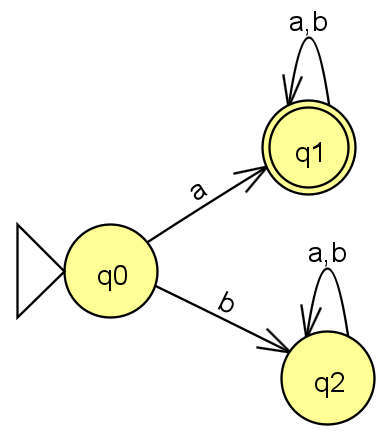
\includegraphics[width=0.2\textwidth]{../../../images/DFAs/ex1_q1.png}



% \vspace{3cm}
% \begin{flushleft}
% أرجو لكم وقتًا ممتعًا.

% الأستاذ محمود اغبارية.
% \end{flushleft}


% \end{document}


\ifwithsols
\title{حل ورقة تمرّن 16: الفئات والكائنات}
\else
\title{ورقة تمرّن 16: الفئات والكائنات}
\fi


\begin{document}

\maketitle
\thispagestyle{fancy}

\begin{enumerate}[itemsep=2em]
    \item
    \begin{enumerate}
        \item أنشئ فئة جديدة باسم \textenglish{Time} تحتوي على ثلاثة حقول عامة (\textenglish{public}) من نوع \textenglish{int}: الساعات (\textenglish{hours})، الدقائق (\textenglish{minutes})، والثواني (\textenglish{seconds}).
        \item في العملية الرئيسية \textenglish{Main}، صرح عن كائنين من نوع \textenglish{Time}: \\
         الأول يمثل الساعة 10:30:15، والثاني يمثل الساعة 08:45:00.
    \end{enumerate}

    \ifwithsols
    \begin{boxSolution}
    \begin{english}
    \begin{minted}{csharp}
// a
class Time
{
    public int hours;
    public int minutes;
    public int seconds;
}

// In Main:
// b
Time t1 = new Time();
t1.hours = 10;
t1.minutes = 30;
t1.seconds = 15;

Time t2 = new Time();
t2.hours = 8;
t2.minutes = 45;
t2.seconds = 0;
    \end{minted}
    \end{english}
    \end{boxSolution}
    \clearpage
    \fi

    % ======================================================
    % 2. إضافة دوال بدون معلمات (Print)
    % ======================================================
    \item
    أضف عملية للفئة \textenglish{Time} باسم \textenglish{Print}. تقوم العملية بطباعة الوقت بالتنسيق التالي: \\
     \textenglish{HH:MM:SS}.
    استدعِ العملية للكائنين \textenglish{t1} و \textenglish{t2} في \textenglish{Main}.
    \begin{boxHint}
    يمكنك مؤقتاً طباعتها بالشكل البسيط: \textenglish{hours + ":" + minutes + ":" + seconds}.
    \end{boxHint}

    \ifwithsols
    \begin{boxSolution}
    \begin{english}
    \begin{minted}{csharp}
public void Print()
{
    Console.WriteLine($"{hours}:{minutes}:{seconds}");
}

// In Main:
t1.Print();
t2.Print();
    \end{minted}
    \end{english}
    \end{boxSolution}
    \clearpage
    \fi

    % ======================================================
    % 3. عملية حسابية (ToSeconds)
    % ======================================================
    \item
    أضف عملية باسم \textenglish{ToSeconds} تعيد إجمالي الوقت بالثواني (عدد صحيح). \\
    استدعِ العملية للكائن \textenglish{t1} واطبع النتيجة.
    \begin{boxHint}
    اضرب الساعات في 3600 والدقائق في 60 واجمعها مع الثواني.
    \end{boxHint}

    \ifwithsols
    \begin{boxSolution}
    \begin{english}
    \begin{minted}{csharp}
public int ToSeconds()
{
    return (hours * 3600) + (minutes * 60) + seconds;
}

// In Main:
Console.WriteLine("Total seconds for t1: " + t1.ToSeconds());
    \end{minted}
    \end{english}
    \end{boxSolution}
    \clearpage
    \fi

    % ======================================================
    % 4. عملية مع معلمات للمقارنة (IsBefore)
    % ======================================================
    \item
    أضف عملية باسم \textenglish{IsBefore(Time other)} تستقبل كائناً آخر من نوع \textenglish{Time}.
    تعيد العملية \textenglish{true} إذا كان وقت الكائن الحالي يسبق وقت الكائن \textenglish{other}، وإلا تعيد \textenglish{false}.
    \begin{boxHint}
    يمكنك استخدام العملية \textenglish{ToSeconds} لتسهيل المقارنة!
    \end{boxHint}

    \ifwithsols
    \begin{boxSolution}
    \begin{english}
    \begin{minted}{csharp}
public bool IsBefore(Time other)
{
    if (other == null) return false;

    return this.ToSeconds() < other.ToSeconds();
}

// In Main:
if (t2.IsBefore(t1))
    Console.WriteLine("t2 is earlier than t1");
    \end{minted}
    \end{english}
    \end{boxSolution}
    \fi
    \clearpage

    % ======================================================
    % 5. عملية البناء (Constructor) والتغليف (Encapsulation)
    % ======================================================
    \item
    \begin{enumerate}
        \item حوّل الحقول الثلاثة (\textenglish{hours, minutes, seconds}) لتكون خاصة (\textenglish{private}).
        \item أضف عملية بناءة (\textenglish{Constructor}) تستقبل الساعات والدقائق والثواني وتهيئ الحقول.
        \item أضف عمليات استرجاع (\textenglish{Getters}): \\
         \textenglish{GetHours(), GetMinutes(), GetSeconds()}.
        \item عدّل كود الـ \textenglish{Main} لإنشاء الكائنات باستخدام عملية البناء في سطر واحد.
    \end{enumerate}

    \ifwithsols
    \begin{boxSolution}
    \begin{english}
    \begin{minted}{csharp}
class Time
{
    // a
    private int hours;
    private int minutes;
    private int seconds;

    // b
    public Time(int hours, int minutes, int seconds)
    {
        this.hours = hours;
        this.minutes = minutes;
        this.seconds = seconds;
    }

    // c
    public int GetHours() { return hours; }
    public int GetMinutes() { return minutes; }
    public int GetSeconds() { return seconds; }

    // ...
}

// In Main:
// d
Time t1 = new Time(10, 30, 15);
    \end{minted}
    \end{english}
    \end{boxSolution}
    \clearpage
    \fi

    % ======================================================
    % 6. عملية معقدة (IncrementTime)
    % ======================================================
    \item
    أضف عملية باسم \textenglish{IncrementTime(int addedSeconds)} تضيف عدداً من الثواني للوقت الحالي.\\
    \textbf{انتبه:} يجب أن تعالج العملية الفائض في الثواني والدقائق.
    \begin{boxExample}
    إذا أضفت ثواني وأصبحت قيمتها 65، يجب أن تزيد الدقائق بمقدار 1 وتصبح الثواني 5. وإذا زادت الساعات عن 23 تعود لـ 0.
    \end{boxExample}

    \ifwithsols
    \begin{boxSolution}
    \begin{english}
    \begin{minted}{csharp}
public void IncrementTime(int addedSeconds)
{
    int totalSeconds = ToSeconds() + addedSeconds;

    // Calculate new time
    this.hours = (totalSeconds / 3600) % 24;
    this.minutes = (totalSeconds % 3600) / 60;
    this.seconds = totalSeconds % 60;
}
    \end{minted}
    \end{english}
    \end{boxSolution}
    \fi
    \clearpage

    \item
    سنقوم الآن ببناء فئة تمثل شخصية في لعبة فيديو.\\
    أنشئ فئة \textenglish{GameCharacter} تحتوي على الحقول الخاصة (\textenglish{private}) التالية:
    \begin{itemize}
        \item \textenglish{string name} (اسم الشخصية)
        \item \textenglish{int health} (نقاط الصحة، الحد الأقصى هو $100 \times level$)
        \item \textenglish{int level} (المستوى، يبدأ بـ 1)
    \end{itemize}
    اكتب عملية بناءة تستقبل اسم الشخصية فقط، وتهيئ الصحة بـ 100 والمستوى بـ 1.

    \ifwithsols
    \begin{boxSolution}
    \begin{english}
    \begin{minted}{csharp}
class GameCharacter
{
    private string name;
    private int health;
    private int level;

    public GameCharacter(string name)
    {
        this.name = name;
        this.health = 100;
        this.level = 1;
    }
}
    \end{minted}
    \end{english}
    \end{boxSolution}
    \clearpage
    \fi

    % ======================================================
    % 8. التغليف وقيود القيم
    % ======================================================
    \item أضف العمليات التالية:
    \begin{enumerate} [itemsep=1em]
    \item أضف عمليات الـ \textenglish{Getters} لجميع الحقول \\
    (\textenglish{GetName, GetHealth, GetLevel}).

    \item
    أضف عملية \textenglish{TakeDamage(int damage)} تقوم بتنقيص الصحة بمقدار الضرر المتلقى. لا يمكن أن تكون الصحة أقل من 0.

    \ifwithsols
    \begin{boxSolution}
    \begin{english}
    \begin{minted}{csharp}
// a
public string GetName() { return name; }
public int GetHealth() { return health; }
public int GetLevel() { return level; }

// b
public void TakeDamage(int damage)
{
    health -= damage;
    if (health < 0)
        health = 0;
}
    \end{minted}
    \end{english}
    \end{boxSolution}
    \clearpage
    \fi

    \item
    أضف عملية \textenglish{bool IsAlive()} تعيد \textenglish{true} إذا كانت صحة الشخصية أكبر من 0.

    \item أضف عملية \textenglish{void PrintStatus()} تطبع اسم الشخصية، مستواها، وصحتها الحالية. وإذا كانت الصحة 0 تطبع أيضاً بجانبها جملة "(مهزوم)".

    \ifwithsols
    \begin{boxSolution}
    \begin{english}
    \begin{minted}{csharp}
// c
public bool IsAlive()
{
    return health > 0;
}

// d
public void PrintStatus()
{
    Console.Write($"Name: {name}, Level: {level}, Health: {health}");
    if (!IsAlive())
    {
        Console.Write(" (Defeated)");
    }
    Console.WriteLine();
}
    \end{minted}
    \end{english}
    \end{boxSolution}
    \clearpage
    \fi

    % ======================================================
    % 10. الشفاء والترقية
    % ======================================================
    \item
    أضف عملية \textenglish{Heal(int amount)} لزيادة الصحة، بشرط ألا تتجاوز الحد الأقصى للصحة وهو ($100 \times level$). ولا يمكن شفاء الشخصية إذا كانت مهزومة.

    \item
    أضف عملية \textenglish{LevelUp()} تقوم بزيادة المستوى بمقدار 1، وتعبئة الصحة بالكامل للحد الأقصى الجديد.

    \ifwithsols
    \begin{boxSolution}
    \begin{english}
    \begin{minted}{csharp}
// e
public void Heal(int amount)
{
    if (!IsAlive()) return; // Must be alive to heal

    int maxHealth = 100 * level;
    health += amount;

    if (health > maxHealth)
        health = maxHealth;
}

// f
public void LevelUp()
{
    level++;
    health = 100 * level; // Fully restore health
    Console.WriteLine($"{name} leveled up to {level}!");
}
    \end{minted}
    \end{english}
    \end{boxSolution}
    \fi

\end{enumerate}
\end{enumerate}

\vspace{1cm}
\begin{flushleft}
أرجو لكم وقتًا ممتعًا.

الأستاذ محمود اغبارية.
\end{flushleft}

\end{document}
